\documentclass[11pt]{article}
\usepackage[margin=1in]{geometry}
\usepackage{amsmath,amssymb}
\usepackage{booktabs,tabularx,array,longtable}
\usepackage{enumitem}
\usepackage{xcolor}
\usepackage[hidelinks]{hyperref}
\usepackage{titlesec}
\usepackage{fancyhdr}
\usepackage{microtype}
\usepackage{lmodern}
\usepackage[T1]{fontenc}
\usepackage{float}
\usepackage{graphicx}
\usepackage{caption}
\usepackage[most]{tcolorbox}
\usepackage{adjustbox}
\usepackage[htt]{hyphenat}
\sloppy

\definecolor{jhublue}{RGB}{0,45,114}
\definecolor{boxgray}{RGB}{244,246,250}
\titleformat{\section}{\large\bfseries\color{jhublue}}{\thesection}{0.6em}{}
\titleformat{\subsection}{\normalsize\bfseries}{\thesubsection}{0.6em}{}
\titleformat{\subsubsection}{\normalsize\itshape}{\thesubsubsection}{0.6em}{}
\setlist{itemsep=2pt,topsep=3pt}
\captionsetup{font=small,labelfont=bf}
\pagestyle{fancy}\fancyhf{}
\cfoot{\small\thepage}
\renewcommand{\headrulewidth}{0.3pt}
\emergencystretch=3em

\newcommand{\PSI}{\mathrm{PSI}}
\newcommand{\file}[1]{\texttt{\small #1}}
\newtcolorbox{summarybox}{colback=boxgray,colframe=jhublue,boxrule=0.6pt,arc=2pt,left=6pt,right=6pt,top=4pt,bottom=4pt,fonttitle=\bfseries,title=Summary}
\newtcolorbox{conceptbox}[1]{colback=white,colframe=jhublue!60,boxrule=0.4pt,arc=2pt,left=6pt,right=6pt,top=3pt,bottom=3pt,fonttitle=\bfseries\small,title={Concept: #1}}
\newtcolorbox{whybox}{colback=boxgray,colframe=gray!50,boxrule=0.4pt,arc=2pt,left=6pt,right=6pt,top=3pt,bottom=3pt}

\lhead{\small Replication of Zhang et al.\ (2026) --- Task 2}
\rhead{\small Sahil, Johns Hopkins University}

\begin{document}

\begin{center}
{\LARGE\bfseries Task 2: Sensitivity of the TWFE estimate\\[2pt] to unobserved confounding}\\[6pt]
{\large Cinelli and Hazlett (2020) omitted-variable-bias analysis}\\[8pt]
Sahil \quad$\cdot$\quad Research Assistant, Johns Hopkins University\\
{\small Prepared for Prof.\ Paul J.\ Ferraro \quad$\cdot$\quad November 2026 \quad$\cdot$\quad All analysis in Stata (StataNow/BE 19.5)}
\end{center}

\begin{summarybox}
\small
\begin{itemize}[leftmargin=12pt]
\item \textbf{The estimate is fragile.} PSI explains only \textbf{0.048\%} of the residual variance in Shannon diversity. An unobserved confounder explaining \textbf{2.2\%} of the residual variance of both PSI and Shannon would reduce the estimate to zero (robustness value). One explaining \textbf{1.2\%} (classical SEs) or \textbf{0.9\%} (county-clustered SEs) would make it statistically insignificant.
\item \textbf{Observed controls are weak benchmarks.} No control explains more than 0.38\% of PSI's residual variance (Water). Observer effort (Duration), by far the strongest predictor of Shannon, explains 0.064\%. A confounder \emph{twice} as strong as Duration leaves the estimate at $-0.0067$, which is no longer significant under the paper's clustered SEs ($t=-1.92$).
\item \textbf{A known confounder is far stronger.} Urban $\times$ year-month trends (Task 1) explain \textbf{12.3\%} of PSI's residual variance: 32 times the most PSI-related control (Water) and 190 times Duration. A hidden factor with half that strength removes the result.
\item \textbf{Under the urban $\times$ year-month specification} the estimate is already insignificant (robustness value for significance = 0).
\end{itemize}
\end{summarybox}

\tableofcontents

%==========================================================================
\section{What Task 2 asks, and why}
Prof.\ Ferraro asked for a \emph{sensitivity analysis to hidden bias (unobservable heterogeneity) of the TWFE analysis}, using Cinelli and Hazlett (2020).

\textbf{Why.} The TWFE estimate is causal only if, after county and year-month fixed effects and the nine controls, \emph{no omitted variable} affects both solar policy and bird diversity. That assumption cannot be tested. Sensitivity analysis instead asks: \emph{how strong would an omitted confounder have to be to change the conclusion, and is a confounder that strong plausible?} Task 1 already identified one strong candidate, the urban--rural divide. This task puts it, and any hypothetical confounder, on a common scale.

%==========================================================================
\section{Concepts}

\begin{conceptbox}{Omitted-variable bias (OVB)}
Suppose the true model also includes a confounder $Z$ that we did not control for. Then our PSI coefficient is off by $\text{bias}=\hat\gamma\,\hat\delta$, where $\hat\gamma$ is $Z$'s effect on Shannon and $\hat\delta$ is how strongly $Z$ moves with PSI. A confounder is dangerous only if it is related to \emph{both}.
\end{conceptbox}

\begin{conceptbox}{Partial $R^2$: the scale of strength}
Cinelli and Hazlett measure a confounder's strength by two \emph{partial $R^2$} values, i.e.\ shares of \emph{residual} variance (what is left after the fixed effects and controls):
\begin{itemize}[leftmargin=12pt]
\item $R^2_{D\sim Z|X}$: the share of PSI's residual variation that $Z$ explains (its link to the treatment);
\item $R^2_{Y\sim Z|D,X}$: the share of Shannon's residual variation that $Z$ explains (its link to the outcome).
\end{itemize}
Both lie between 0 and 1, so they are easy to compare with observed variables.
\end{conceptbox}

\begin{conceptbox}{Bias formula and robustness value}
Given the two strengths, the bias is (C\&H eq.~12)
\[
|\text{bias}| = \text{se}(\hat\beta)\sqrt{\text{df}}\;\sqrt{\frac{R^2_{Y\sim Z|D,X}\,R^2_{D\sim Z|X}}{1-R^2_{D\sim Z|X}}}.
\]
The \textbf{robustness value} $RV$ is the strength a confounder needs, \emph{equally} on both axes, to bring the estimate to zero (eq.~18). $RV_\alpha$ is the strength needed to make it statistically insignificant (eqs.~19--20). The \textbf{partial $R^2$ of PSI with Shannon}, $R^2_{Y\sim D|X}$, is the extreme case: a confounder explaining \emph{all} the leftover outcome variance needs only this much of the treatment to explain the estimate away.
\end{conceptbox}

\begin{conceptbox}{Benchmarking}
Raw numbers like ``2\%'' are hard to judge. Cinelli and Hazlett compare them with an observed covariate: ``a confounder $k$ times as strong as Duration'' (eqs.~21--22). This is done with formal \emph{bounds}, not by naively plugging in Duration's own $R^2$, which can mislead (their Section 6.2).
\end{conceptbox}

%==========================================================================
\section{Workflow}
\begin{table}[H]\centering\small
\caption{Steps in \file{02\_Task2\_Sensitivity/code/2\_1\_sensitivity\_analysis.do}}
\begin{tabularx}{\linewidth}{c>{\raggedright\arraybackslash}X>{\raggedright\arraybackslash}X}
\toprule
Step & What and why & Output\\
\midrule
A & Re-estimate the TWFE model with classical SEs to obtain the exact $t$ and residual df. Compute $R^2_{Y\sim D|X}$, $RV$ and $RV_{\alpha=0.05}$ & \file{tables/2\_1\_robustness\_values.csv}\\
B & Benchmark bounds: confounders 1, 2 and 3 times as strong as each of the nine controls; adjusted estimate and $t$ & \file{tables/2\_1\_benchmark\_bounds.csv}\\
C & Group benchmark: a confounder as strong as urban $\times$ year-month trends ($k=0.25, 0.5, 1$) & same file\\
D & Clustered-inference variant, because the paper uses county-clustered SEs & both tables\\
E & Contour plots of the adjusted estimate and $t$ & \file{figures/2\_1\_contour\_*.pdf}\\
F & Cross-check against the official \file{sensemakr} package & log\\
\bottomrule
\end{tabularx}
\end{table}
Each step is run for two specifications: \textbf{S1}, the paper's baseline (county + year-month FE), and \textbf{S2}, urban $\times$ year-month FE from Task 1.

\subsection{Two technical choices}
\textbf{Fixed effects.} The model has about 2,460 fixed effects, too many for \file{sensemakr} to include as dummies in StataBE. By the Frisch--Waugh--Lovell theorem, partialling the fixed effects out of every variable leaves the PSI coefficient unchanged. All partial $R^2$s are therefore computed from \file{reghdfe} $t$-statistics using its \emph{exact} residual degrees of freedom ($\text{df}=43{,}898$). The fixed effects themselves count as observed controls.

\textbf{Clustered standard errors.} The Cinelli--Hazlett formulas assume classical SEs, while the paper clusters by county. The partial $R^2$s measure \emph{how strong} a confounder is, which is an identification question independent of the SEs. So they are always computed from the classical model. Only the significance threshold changes: it is scaled by $\lambda=\text{SE}_{\text{clustered}}/\text{SE}_{\text{classical}}=1.34$. Equivalently, an adjusted $t$ is divided by $\lambda$. Plugging the clustered $t$ and $G-1$ degrees of freedom straight into the formulas would be wrong: it changes the partial $R^2$ itself, and gives a \emph{larger} robustness value despite a smaller $t$. I recommend confirming this choice with Prof.\ Ferraro.

%==========================================================================
\section{Results}

\subsection{Robustness values}
\begin{table}[H]\centering\small
\caption{Sensitivity statistics (\file{tables/2\_1\_robustness\_values.csv})}\label{tab:rv}
\begin{tabular}{lcc}
\toprule
& S1: paper baseline & S2: urban $\times$ YM FE\\
\midrule
PSI estimate & $-0.01253$ & $-0.00268$\\
$t$ (classical / clustered) & $-4.58$ / $-3.43$ & $-0.92$ / $-0.72$\\
Residual df & 43,898 & 43,779\\
$R^2_{Y\sim D|X}$ (partial $R^2$ of PSI with Shannon) & 0.048\% & 0.002\%\\
$RV$ (estimate to zero) & \textbf{2.16\%} & 0.44\%\\
$RV_{\alpha=0.05}$, classical SE & \textbf{1.24\%} & 0\\
$RV_{\alpha=0.05}$, clustered SE ($\lambda=1.34$) & \textbf{0.93\%} & 0\\
\bottomrule
\end{tabular}
\end{table}
\noindent\textbf{Interpretation.} A confounder explaining 2.2\% of the residual variance of both PSI and Shannon removes the estimate entirely. One explaining about 1\% removes its significance. In the extreme case, a confounder explaining all of Shannon's residual variance needs to explain only 0.048\% of PSI's. Under S2 the estimate is already insignificant, so no confounder is needed.

\subsection{Benchmarks: how strong are the variables we can see?}
\begin{table}[H]\centering\small
\caption{Bounds for confounders $k$ times as strong as an observed variable (S1; \file{tables/2\_1\_benchmark\_bounds.csv})}\label{tab:bounds}
\begin{adjustbox}{max width=\linewidth}
\begin{tabular}{lcccccc}
\toprule
Benchmark & $k$ & $R^2_{D\sim Z|X}$ & $R^2_{Y\sim Z|D,X}$ & Adjusted est. & Adj.\ $t$ (classical) & Adj.\ $t$ (clustered)\\
\midrule
Duration (effort) & 1 & 0.06\% & 4.0\% & $-0.0096$ & $-3.59$ & $-2.69$\\
Duration & 2 & 0.13\% & 8.0\% & $-0.0067$ & $-2.56$ & $\mathbf{-1.92}$\\
Duration & 3 & 0.19\% & 12.1\% & $-0.0038$ & $-1.49$ & $-1.11$\\
Water (most PSI-related) & 1 & 0.38\% & 0.008\% & $-0.0122$ & $-4.46$ & $-3.34$\\
Water & 3 & 1.14\% & 0.023\% & $-0.0116$ & $-4.22$ & $-3.15$\\
Other seven controls & 1--3 & $\le$0.66\% & $<$0.1\% & $-0.0120$ to $-0.0125$ & --- & ---\\
\midrule
Urban $\times$ YM trends & 0.25 & 3.5\% & 0.19\% & $-0.0077$ & $-2.78$ & $-2.08$\\
Urban $\times$ YM trends & \textbf{0.5} & 7.0\% & 0.39\% & $\mathbf{-0.0027}$ & $-0.96$ & $-0.72$\\
Urban $\times$ YM trends & 1 & 14.0\% & 0.79\% & $+0.0081$ & $+2.75$ & $+2.05$\\
\bottomrule
\end{tabular}
\end{adjustbox}
\par\smallskip\footnotesize Observed strengths: Duration explains 0.064\% of PSI and 3.9\% of Shannon; Water 0.38\% of PSI and 0.008\% of Shannon; urban $\times$ YM trends 12.3\% of PSI and 0.59\% of Shannon.
\end{table}

\begin{whybox}\small
\textbf{Reading Table~\ref{tab:bounds}.} Judged against the paper's own controls, the result looks reasonably robust. Even a confounder three times as strong as any single control leaves a negative point estimate, because none of the controls is strongly related to PSI. But the controls are a weak yardstick. Urban $\times$ month trends, a factor we can actually measure, are 32 times more strongly tied to PSI than the most PSI-related control (Water) and 190 times more than Duration. A hidden factor with \emph{half} that strength wipes out the estimate. With a quarter of it, the estimate is still significant. When the urban trends are actually added to the model (Task 1), the estimate becomes $-0.0027$, the same as the $k=0.5$ bound. The question is therefore not whether a confounder of the required size \emph{could} exist; one demonstrably does.
\end{whybox}

\subsection{Contour plots}
\begin{figure}[H]\centering
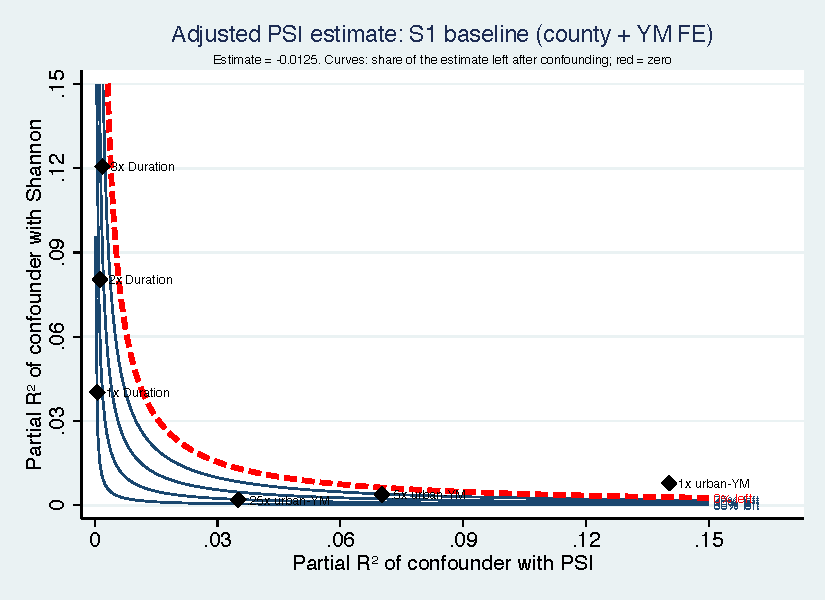
\includegraphics[width=0.49\linewidth]{../figures/2_1_contour_estimate_S1.pdf}\hfill
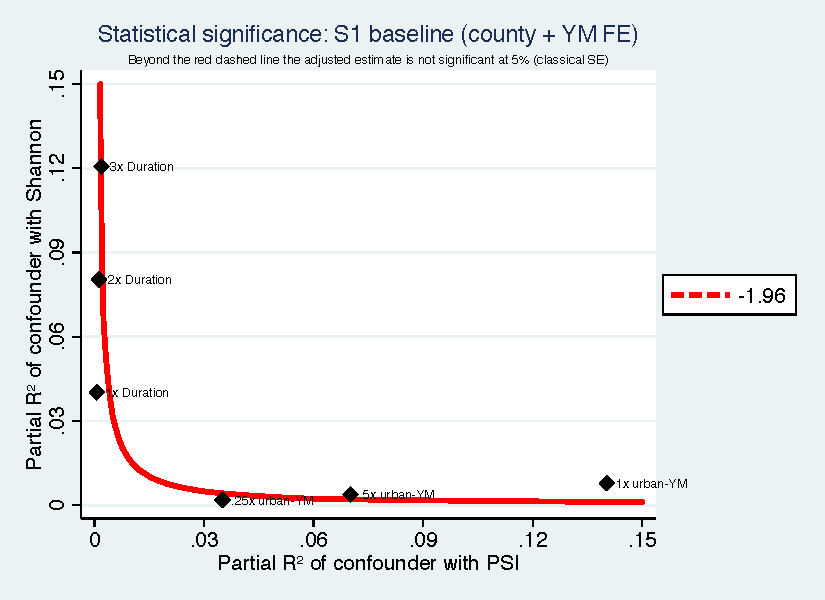
\includegraphics[width=0.49\linewidth]{../figures/2_1_contour_tvalue_S1.pdf}
\caption{S1 (paper baseline). Left: each curve shows the confounder strengths that leave a given share of the estimate (red dashed: zero). Right: beyond the red line the adjusted estimate is no longer significant at 5\%. Diamonds: bounds for confounders $k\times$ Duration (near the vertical axis) and $k\times$ urban $\times$ YM trends (along the bottom).}
\end{figure}
\begin{figure}[H]\centering
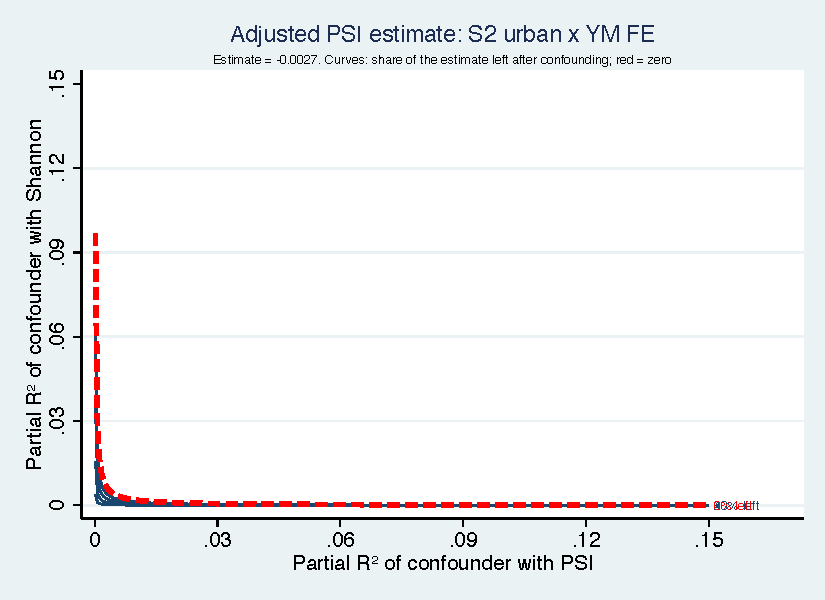
\includegraphics[width=0.6\linewidth]{../figures/2_1_contour_estimate_S2.pdf}
\caption{S2 (urban $\times$ year-month FE). The estimate is already insignificant (so there is no significance line to plot), and small confounders move it to zero.}
\end{figure}

\subsection{Cross-check with \file{sensemakr}}
The official \file{sensemakr} package, run on fixed-effect-demeaned data, gives $RV=2.16\%$, identical to ours. It gives $RV_\alpha=1.27\%$ against our 1.24\%; the small difference arises because its degrees of freedom (46,360) ignore the absorbed fixed effects, while ours are exact (43,898). Its Duration bounds ($-0.0096$, $-0.0067$, $-0.0038$) match Table~\ref{tab:bounds} exactly. An earlier, independent Python implementation (another session; its draft report is \file{Stata Analysis/Replication/Report/Task2\_Report.pdf}) reported the same robustness value, 2.2\%.

%==========================================================================
\section{Conclusions}
\begin{enumerate}
\item The paper's estimate can be explained away by a confounder explaining about 2\% of the residual variance of both PSI and bird diversity, and made insignificant by one explaining about 1\%.
\item Relative to the paper's own controls this looks robust, but the controls are weakly related to PSI and are a poor benchmark.
\item The urban--rural trend identified in Task 1 is a real, measured confounder whose strength exceeds what is needed. That is consistent with the estimate collapsing once it is controlled for.
\item The sensitivity analysis and the Task 1 diagnostics therefore point the same way: the TWFE association is not robust to plausible confounding.
\end{enumerate}

\section{How to reproduce}
In Stata, type
\begin{quote}\small\texttt{do ".../02\_Task2\_Sensitivity/code/2\_0\_run\_task2.do"}\end{quote} This needs \file{01\_Task1\_Replication/data/analysis\_sample.dta}, built by Task 1. The log is \file{logs/2\_1\_sensitivity\_analysis.log}.

\section*{References}
{\small
\begin{itemize}[leftmargin=12pt,label={}]
\item Cinelli, C.\ and Hazlett, C.\ (2020). Making sense of sensitivity: extending omitted variable bias. \textit{Journal of the Royal Statistical Society: Series B}, 82(1), 39--67.
\item Cinelli, C., Ferwerda, J.\ and Hazlett, C.\ \file{sensemakr}: sensitivity analysis tools for OLS (Stata, R and Python packages).
\item Frisch, R.\ and Waugh, F.\ V.\ (1933). Partial time regressions as compared with individual trends. \textit{Econometrica}, 1(4), 387--401; Lovell, M.\ C.\ (1963). Seasonal adjustment of economic time series and multiple regression analysis. \textit{JASA}, 58(304), 993--1010.
\item Zhang, H.\ et al.\ (2026). China's solar expansion policy reduces bird diversity. \textit{Science}, 393, 831.
\end{itemize}}

\end{document}
